% Für Bindekorrektur als optionales Argument "BCORfaktormitmaßeinheit", dann
% sieht auch Option "twoside" vernünftig aus
% Näheres zu "scrartcl" bzw. "scrreprt" und "scrbook" siehe KOMA-Skript Doku
\documentclass[12pt,a4paper,titlepage,headinclude,bibtotoc]{scrartcl}


%---- Allgemeine Layout Einstellungen ------------------------------------------

% Für Kopf und Fußzeilen, siehe auch KOMA-Skript Doku
\usepackage[komastyle]{scrpage2}
\pagestyle{scrheadings}
\setheadsepline{0.5pt}[\color{black}]
\automark[section]{chapter}


%Einstellungen für Figuren- und Tabellenbeschriftungen
\setkomafont{captionlabel}{\sffamily\bfseries}
\setcapindent{0em}


%---- Weitere Pakete -----------------------------------------------------------
% Die Pakete sind alle in der TeX Live Distribution enthalten. Wichtige Adressen
% www.ctan.org, www.dante.de

% Sprachunterstützung
\usepackage[ngerman]{babel}

% Benutzung von Umlauten direkt im Text
% entweder "latin1" oder "utf8"
\usepackage[utf8]{inputenc}

% Pakete mit Mathesymbolen und zur Beseitigung von Schwächen der Mathe-Umgebung
\usepackage{latexsym,exscale,stmaryrd,amssymb,amsmath}

% Weitere Symbole
\usepackage[nointegrals]{wasysym}
\usepackage{eurosym}

% Anderes Literaturverzeichnisformat
%\usepackage[square,sort&compress]{natbib}

% Für Farbe
\usepackage{color}

% Zur Graphikausgabe
%Beipiel: \includegraphics[width=\textwidth]{grafik.png}
\usepackage{graphicx}

% Text umfließt Graphiken und Tabellen
% Beispiel:
% \begin{wrapfigure}[Zeilenanzahl]{"l" oder "r"}{breite}
%   \centering
%   \includegraphics[width=...]{grafik}
%   \caption{Beschriftung} 
%   \label{fig:grafik}
% \end{wrapfigure}
\usepackage{wrapfig}

% Mehrere Abbildungen nebeneinander
% Beispiel:
% \begin{figure}[htb]
%   \centering
%   \subfigure[Beschriftung 1\label{fig:label1}]
%   {\includegraphics[width=0.49\textwidth]{grafik1}}
%   \hfill
%   \subfigure[Beschriftung 2\label{fig:label2}]
%   {\includegraphics[width=0.49\textwidth]{grafik2}}
%   \caption{Beschriftung allgemein}
%   \label{fig:label-gesamt}
% \end{figure}
\usepackage{subfigure}

% Caption neben Abbildung
% Beispiel:
% \sidecaptionvpos{figure}{"c" oder "t" oder "b"}
% \begin{SCfigure}[rel. Breite (normalerweise = 1)][hbt]
%   \centering
%   \includegraphics[width=0.5\textwidth]{grafik.png}
%   \caption{Beschreibung}
%   \label{fig:}
% \end{SCfigure}
\usepackage{sidecap}

% Befehl für "Entspricht"-Zeichen
\newcommand{\corresponds}{\ensuremath{\mathrel{\widehat{=}}}}
% Befehl für Errorfunction
\newcommand{\erf}[1]{\text{ erf}\ensuremath{\left( #1 \right)}}

%Fußnoten zwingend auf diese Seite setzen
\interfootnotelinepenalty=1000

%Für chemische Formeln (von www.dante.de)
%% Anpassung an LaTeX(2e) von Bernd Raichle
\makeatletter
\DeclareRobustCommand{\chemical}[1]{%
  {\(\m@th
   \edef\resetfontdimens{\noexpand\)%
       \fontdimen16\textfont2=\the\fontdimen16\textfont2
       \fontdimen17\textfont2=\the\fontdimen17\textfont2\relax}%
   \fontdimen16\textfont2=2.7pt \fontdimen17\textfont2=2.7pt
   \mathrm{#1}%
   \resetfontdimens}}
\makeatother

%Honecker-Kasten mit $$\shadowbox{$xxxx$}$$
\usepackage{fancybox}

%SI-Package
\usepackage{siunitx}

%keine Einrückung, wenn Latex doppelte Leerzeile
\parindent0pt

%Bibliography \bibliography{literatur} und \cite{gerthsen}
%\usepackage{cite}
\usepackage{babelbib}
\selectbiblanguage{ngerman}

\begin{document}

\begin{titlepage}
\centering
\textsc{\Large Anfängerpraktikum der Fakultät für
  Physik,\\[1.5ex] Universität Göttingen}

\vspace*{4.2cm}

\rule{\textwidth}{1pt}\\[0.5cm]
{\huge \bfseries
  Wechselstromwiderstände\\[1.5ex]
  Protokoll}\\[0.5cm]
\rule{\textwidth}{1pt}

\vspace*{2.5cm}

\begin{Large}
\begin{tabular}{ll}
Praktikant: & Felix Kurtz\\
Versuchspartner & Michael Lohmann\\
 E-Mail: &  felix.kurtz@stud.uni-goettingen.de\\
 Betreuer: & Björn Klaas\\
 Versuchsdatum: & 08.09.2014\\
\end{tabular}
\end{Large}

\vspace*{0.8cm}

\begin{Large}
\fbox{
  \begin{minipage}[t][2.5cm][t]{6cm} 
   eingegangen am:
  \end{minipage}
}
\end{Large}

\end{titlepage}

\tableofcontents

\newpage

\section{Einleitung}
\label{sec:einleitung}
Bei diesem Versuch sollen induktive und kapazitive Widerstände und die damit verbundene Phasenverschiebung zwischen Strom und Spannung untersucht werden.
%bla bla

\section{Theorie}
\label{sec:theorie}
\subsection{Induktiver Widerstand}

\begin{align}
	X_L=i\omega L \,.
\end{align}

Außerdem besitzen Spulen meist einen nicht zu vernachlässigenden ohmschen Widerstand $R_L$, da sie aus sehr langem Draht bestehen.

\subsection{Kapazitiver Widerstand}

\begin{align}
	X_C=-i\frac{1}{\omega C} \,.
\end{align}

\subsection{Impedanz und Zeigerdiagramm}
Impedanz
\begin{align}
	Z=R+X_C+X_L \,.
\end{align}
Scheinwiderstand
\begin{align}
	|Z|=\sqrt{R^2+\left(\omega L - \frac{1}{\omega C}\right)^2} \,.
\end{align}

Minimaler Widerstand bei der Resonanzfrequenz
\begin{align}
	\omega_R=\sqrt{\frac{1}{LC}} \,.
\end{align}

\subsection{Parallelschaltung}

\subsection{Effektivwerte}
Als \textit{Effektivwert} eines Wechselstroms bezeichnet man den Wert, bei dem bei Gleichstrom die gleich Leistung abgegeben würde.
Für eine Sinus-förmige Spannung der Amplitude $U_0$ ergibt sich somit
\begin{align}
	U_\text{eff}=\sqrt{\frac{1}{2}}\cdot U_0 \,.
\end{align}
Analoges gilt für den Strom.
Vom Multimeter, welches Wechselstrom misst, wird der Effektivwert und nicht die Amplitude der Messgröße angezeigt.
                                                                                                                                                                      
\section{Durchführung}
\label{sec:durchfuehrung}

Zuerst wird der \textbf{Serienresonanzkreis} aus Abb. \eqref{fig:serie} aufgebaut.
Dabei wird das Oszilloskop so angeschlossen und eingestellt, dass die Phasenverschiebung zwischen Strom und Spannung abgelesen werden kann.
Zur ersten Messung überbrückt man den Kondensator, indem man den Schalter schließt.
Nun wird für mindestens 10 Frequenzen Spannung und Strom sowie dren Phasenverschiebung gemessen.
Daraus kann man später die Induktivität der Spule sowie den ohmschen Widerstand berechnen.\\
Die nächsten Messungen finden mit dem Kondensator statt, der Schalter wird also geöffnet.
In Abhängigkeit der Frequenz werden jetzt der Strom $I$, die Spannung $U$ sowie die Teilspannungen $U_C$ und $U_{L+R}$ und die Phasenverschiebung $\varphi$ gemessen.
Dabei sollen möglichst viele Messungen in der Nähe der Resonanzfrequenz $\omega_R$ durchgeführt werden.\\
Als nächstes wird die Schaltung zu einem \textbf{Parallelkreis} aus Spule und Kondensator umgebaut.
Wieder wird die Spannung und der Strom in Abhängigkeit der Frequenz gemessen.
Hier liegt der Fokus wie zuvor auf der Resonanzfrequenz.\\

Zum Schluss misst man mit dem Multimeter den Innenwiderstand des Amperemeters und die ohmschen Widerstände $R_\Omega$ sowie $R_L$.
Außerdem werden die Kapazität des Kondensators gemessen und die Spulendaten notiert. 

\section{Auswertung}
\label{sec:auswertung}
\subsection{Widerstand und Spule in Reihe}
\begin{figure}[!htb]
	\centering
	% GNUPLOT: LaTeX picture with Postscript
\begingroup
  \makeatletter
  \providecommand\color[2][]{%
    \GenericError{(gnuplot) \space\space\space\@spaces}{%
      Package color not loaded in conjunction with
      terminal option `colourtext'%
    }{See the gnuplot documentation for explanation.%
    }{Either use 'blacktext' in gnuplot or load the package
      color.sty in LaTeX.}%
    \renewcommand\color[2][]{}%
  }%
  \providecommand\includegraphics[2][]{%
    \GenericError{(gnuplot) \space\space\space\@spaces}{%
      Package graphicx or graphics not loaded%
    }{See the gnuplot documentation for explanation.%
    }{The gnuplot epslatex terminal needs graphicx.sty or graphics.sty.}%
    \renewcommand\includegraphics[2][]{}%
  }%
  \providecommand\rotatebox[2]{#2}%
  \@ifundefined{ifGPcolor}{%
    \newif\ifGPcolor
    \GPcolortrue
  }{}%
  \@ifundefined{ifGPblacktext}{%
    \newif\ifGPblacktext
    \GPblacktexttrue
  }{}%
  % define a \g@addto@macro without @ in the name:
  \let\gplgaddtomacro\g@addto@macro
  % define empty templates for all commands taking text:
  \gdef\gplbacktext{}%
  \gdef\gplfronttext{}%
  \makeatother
  \ifGPblacktext
    % no textcolor at all
    \def\colorrgb#1{}%
    \def\colorgray#1{}%
  \else
    % gray or color?
    \ifGPcolor
      \def\colorrgb#1{\color[rgb]{#1}}%
      \def\colorgray#1{\color[gray]{#1}}%
      \expandafter\def\csname LTw\endcsname{\color{white}}%
      \expandafter\def\csname LTb\endcsname{\color{black}}%
      \expandafter\def\csname LTa\endcsname{\color{black}}%
      \expandafter\def\csname LT0\endcsname{\color[rgb]{1,0,0}}%
      \expandafter\def\csname LT1\endcsname{\color[rgb]{0,1,0}}%
      \expandafter\def\csname LT2\endcsname{\color[rgb]{0,0,1}}%
      \expandafter\def\csname LT3\endcsname{\color[rgb]{1,0,1}}%
      \expandafter\def\csname LT4\endcsname{\color[rgb]{0,1,1}}%
      \expandafter\def\csname LT5\endcsname{\color[rgb]{1,1,0}}%
      \expandafter\def\csname LT6\endcsname{\color[rgb]{0,0,0}}%
      \expandafter\def\csname LT7\endcsname{\color[rgb]{1,0.3,0}}%
      \expandafter\def\csname LT8\endcsname{\color[rgb]{0.5,0.5,0.5}}%
    \else
      % gray
      \def\colorrgb#1{\color{black}}%
      \def\colorgray#1{\color[gray]{#1}}%
      \expandafter\def\csname LTw\endcsname{\color{white}}%
      \expandafter\def\csname LTb\endcsname{\color{black}}%
      \expandafter\def\csname LTa\endcsname{\color{black}}%
      \expandafter\def\csname LT0\endcsname{\color{black}}%
      \expandafter\def\csname LT1\endcsname{\color{black}}%
      \expandafter\def\csname LT2\endcsname{\color{black}}%
      \expandafter\def\csname LT3\endcsname{\color{black}}%
      \expandafter\def\csname LT4\endcsname{\color{black}}%
      \expandafter\def\csname LT5\endcsname{\color{black}}%
      \expandafter\def\csname LT6\endcsname{\color{black}}%
      \expandafter\def\csname LT7\endcsname{\color{black}}%
      \expandafter\def\csname LT8\endcsname{\color{black}}%
    \fi
  \fi
  \setlength{\unitlength}{0.0500bp}%
  \begin{picture}(7200.00,5040.00)%
    \gplgaddtomacro\gplbacktext{%
      \csname LTb\endcsname%
      \put(946,704){\makebox(0,0)[r]{\strut{} 0}}%
      \put(946,1213){\makebox(0,0)[r]{\strut{} 0.2}}%
      \put(946,1722){\makebox(0,0)[r]{\strut{} 0.4}}%
      \put(946,2231){\makebox(0,0)[r]{\strut{} 0.6}}%
      \put(946,2740){\makebox(0,0)[r]{\strut{} 0.8}}%
      \put(946,3248){\makebox(0,0)[r]{\strut{} 1}}%
      \put(946,3757){\makebox(0,0)[r]{\strut{} 1.2}}%
      \put(946,4266){\makebox(0,0)[r]{\strut{} 1.4}}%
      \put(946,4775){\makebox(0,0)[r]{\strut{} 1.6}}%
      \put(1078,484){\makebox(0,0){\strut{} 0}}%
      \put(1651,484){\makebox(0,0){\strut{} 1}}%
      \put(2223,484){\makebox(0,0){\strut{} 2}}%
      \put(2796,484){\makebox(0,0){\strut{} 3}}%
      \put(3368,484){\makebox(0,0){\strut{} 4}}%
      \put(3941,484){\makebox(0,0){\strut{} 5}}%
      \put(4513,484){\makebox(0,0){\strut{} 6}}%
      \put(5086,484){\makebox(0,0){\strut{} 7}}%
      \put(5658,484){\makebox(0,0){\strut{} 8}}%
      \put(6231,484){\makebox(0,0){\strut{} 9}}%
      \put(6803,484){\makebox(0,0){\strut{} 10}}%
      \put(176,2739){\rotatebox{-270}{\makebox(0,0){\strut{}$|Z|^2$ [(k$\Omega )^2$]}}}%
      \put(3940,154){\makebox(0,0){\strut{}$\omega^2$ [(kHz)$^2$]}}%
    }%
    \gplgaddtomacro\gplfronttext{%
      \csname LTb\endcsname%
      \put(3454,4602){\makebox(0,0)[r]{\strut{}Messwerte}}%
      \csname LTb\endcsname%
      \put(3454,4382){\makebox(0,0)[r]{\strut{}Regressionsgerade}}%
    }%
    \gplbacktext
    \put(0,0){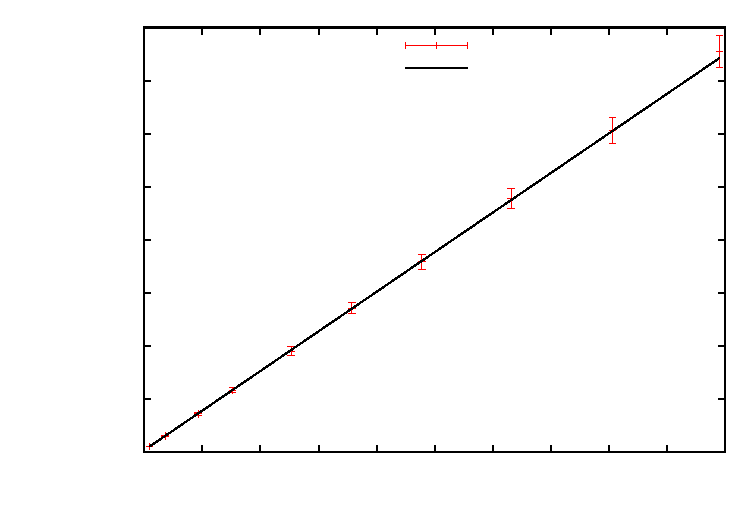
\includegraphics{messung1}}%
    \gplfronttext
  \end{picture}%
\endgroup

	\caption{Quadrat der Impedanz als Funktion der Kreisfrequenz}
	\label{fig:messung1}
\end{figure}

\begin{align}
	L&=(386.3\pm 0.6)\,\si{\milli\henry}\\
	R_\text{ges}&=(77.3 \pm 1.1)\,\si{\ohm}
\end{align}
\subsection{RLC-Serienschaltung}
\begin{figure}[!htb]
	\centering
	% GNUPLOT: LaTeX picture with Postscript
\begingroup
  \makeatletter
  \providecommand\color[2][]{%
    \GenericError{(gnuplot) \space\space\space\@spaces}{%
      Package color not loaded in conjunction with
      terminal option `colourtext'%
    }{See the gnuplot documentation for explanation.%
    }{Either use 'blacktext' in gnuplot or load the package
      color.sty in LaTeX.}%
    \renewcommand\color[2][]{}%
  }%
  \providecommand\includegraphics[2][]{%
    \GenericError{(gnuplot) \space\space\space\@spaces}{%
      Package graphicx or graphics not loaded%
    }{See the gnuplot documentation for explanation.%
    }{The gnuplot epslatex terminal needs graphicx.sty or graphics.sty.}%
    \renewcommand\includegraphics[2][]{}%
  }%
  \providecommand\rotatebox[2]{#2}%
  \@ifundefined{ifGPcolor}{%
    \newif\ifGPcolor
    \GPcolortrue
  }{}%
  \@ifundefined{ifGPblacktext}{%
    \newif\ifGPblacktext
    \GPblacktexttrue
  }{}%
  % define a \g@addto@macro without @ in the name:
  \let\gplgaddtomacro\g@addto@macro
  % define empty templates for all commands taking text:
  \gdef\gplbacktext{}%
  \gdef\gplfronttext{}%
  \makeatother
  \ifGPblacktext
    % no textcolor at all
    \def\colorrgb#1{}%
    \def\colorgray#1{}%
  \else
    % gray or color?
    \ifGPcolor
      \def\colorrgb#1{\color[rgb]{#1}}%
      \def\colorgray#1{\color[gray]{#1}}%
      \expandafter\def\csname LTw\endcsname{\color{white}}%
      \expandafter\def\csname LTb\endcsname{\color{black}}%
      \expandafter\def\csname LTa\endcsname{\color{black}}%
      \expandafter\def\csname LT0\endcsname{\color[rgb]{1,0,0}}%
      \expandafter\def\csname LT1\endcsname{\color[rgb]{0,1,0}}%
      \expandafter\def\csname LT2\endcsname{\color[rgb]{0,0,1}}%
      \expandafter\def\csname LT3\endcsname{\color[rgb]{1,0,1}}%
      \expandafter\def\csname LT4\endcsname{\color[rgb]{0,1,1}}%
      \expandafter\def\csname LT5\endcsname{\color[rgb]{1,1,0}}%
      \expandafter\def\csname LT6\endcsname{\color[rgb]{0,0,0}}%
      \expandafter\def\csname LT7\endcsname{\color[rgb]{1,0.3,0}}%
      \expandafter\def\csname LT8\endcsname{\color[rgb]{0.5,0.5,0.5}}%
    \else
      % gray
      \def\colorrgb#1{\color{black}}%
      \def\colorgray#1{\color[gray]{#1}}%
      \expandafter\def\csname LTw\endcsname{\color{white}}%
      \expandafter\def\csname LTb\endcsname{\color{black}}%
      \expandafter\def\csname LTa\endcsname{\color{black}}%
      \expandafter\def\csname LT0\endcsname{\color{black}}%
      \expandafter\def\csname LT1\endcsname{\color{black}}%
      \expandafter\def\csname LT2\endcsname{\color{black}}%
      \expandafter\def\csname LT3\endcsname{\color{black}}%
      \expandafter\def\csname LT4\endcsname{\color{black}}%
      \expandafter\def\csname LT5\endcsname{\color{black}}%
      \expandafter\def\csname LT6\endcsname{\color{black}}%
      \expandafter\def\csname LT7\endcsname{\color{black}}%
      \expandafter\def\csname LT8\endcsname{\color{black}}%
    \fi
  \fi
  \setlength{\unitlength}{0.0500bp}%
  \begin{picture}(7200.00,5040.00)%
    \gplgaddtomacro\gplbacktext{%
      \csname LTb\endcsname%
      \put(946,704){\makebox(0,0)[r]{\strut{} 0}}%
      \put(946,1156){\makebox(0,0)[r]{\strut{} 0.2}}%
      \put(946,1609){\makebox(0,0)[r]{\strut{} 0.4}}%
      \put(946,2061){\makebox(0,0)[r]{\strut{} 0.6}}%
      \put(946,2513){\makebox(0,0)[r]{\strut{} 0.8}}%
      \put(946,2966){\makebox(0,0)[r]{\strut{} 1}}%
      \put(946,3418){\makebox(0,0)[r]{\strut{} 1.2}}%
      \put(946,3870){\makebox(0,0)[r]{\strut{} 1.4}}%
      \put(946,4323){\makebox(0,0)[r]{\strut{} 1.6}}%
      \put(946,4775){\makebox(0,0)[r]{\strut{} 1.8}}%
      \put(1078,484){\makebox(0,0){\strut{} 0}}%
      \put(1794,484){\makebox(0,0){\strut{} 0.5}}%
      \put(2509,484){\makebox(0,0){\strut{} 1}}%
      \put(3225,484){\makebox(0,0){\strut{} 1.5}}%
      \put(3941,484){\makebox(0,0){\strut{} 2}}%
      \put(4656,484){\makebox(0,0){\strut{} 2.5}}%
      \put(5372,484){\makebox(0,0){\strut{} 3}}%
      \put(6087,484){\makebox(0,0){\strut{} 3.5}}%
      \put(6803,484){\makebox(0,0){\strut{} 4}}%
      \put(176,2739){\rotatebox{-270}{\makebox(0,0){\strut{}Impedanz [k$\Omega$]}}}%
      \put(3940,154){\makebox(0,0){\strut{}Kreisfrequenz [kHz]}}%
    }%
    \gplgaddtomacro\gplfronttext{%
      \csname LTb\endcsname%
      \put(5816,4602){\makebox(0,0)[r]{\strut{}Messwerte}}%
      \csname LTb\endcsname%
      \put(5816,4382){\makebox(0,0)[r]{\strut{}Fit}}%
    }%
    \gplbacktext
    \put(0,0){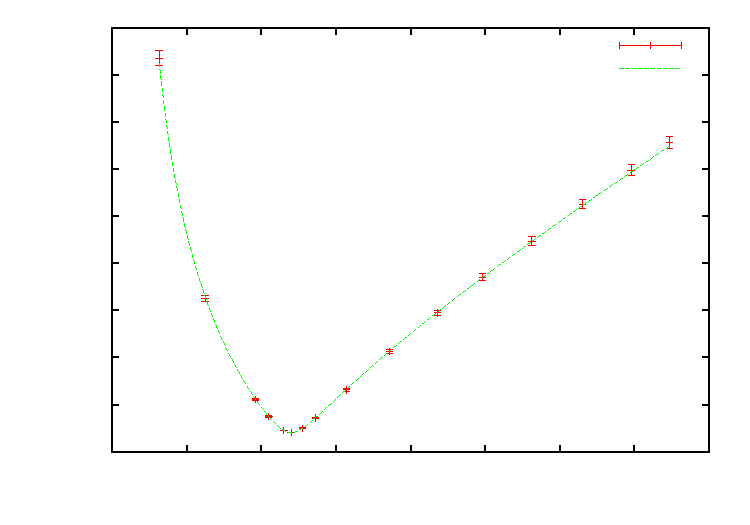
\includegraphics{messung2}}%
    \gplfronttext
  \end{picture}%
\endgroup

	\caption{Impedanz des Serienresonanzkreis als Funktion der Kreisfrequenz}
	\label{fig:messung2}
\end{figure}
Aus
\begin{align}
	R &= (80.9 \pm 0.5)\,\si{\ohm}\\
	L &= (386.1 \pm 1.0)\,\si{\milli\henry}\\
	C &= (1.799 \pm 0.005)\,\si{\micro\farad}
\end{align}
Mittelwerte aus allen Daten:
\begin{align}
\overline L&=(386.2 \pm 0.6)\si{\milli\henry}\\
\overline R&=(80.2836 \pm 0.455183)\,\si{\ohm}
\end{align}
\begin{align}
\omega_\text{LC}&=\frac{1}{\sqrt{LC}}\\
\sigma_{\omega_\text{LC}}&=\frac{\sqrt{\frac{\sigma_{L}^{2}}{L^{2}} + \frac{\sigma_{C}^{2}}{C^{2}}}}{2 \cdot \sqrt{C} \cdot \sqrt{L}}\\
\omega_\text{LC}&=(1199.9 \pm 2.3)\,\si{\hertz}
\end{align}
\begin{figure}[!htb]
	\centering
	% GNUPLOT: LaTeX picture with Postscript
\begingroup
  \makeatletter
  \providecommand\color[2][]{%
    \GenericError{(gnuplot) \space\space\space\@spaces}{%
      Package color not loaded in conjunction with
      terminal option `colourtext'%
    }{See the gnuplot documentation for explanation.%
    }{Either use 'blacktext' in gnuplot or load the package
      color.sty in LaTeX.}%
    \renewcommand\color[2][]{}%
  }%
  \providecommand\includegraphics[2][]{%
    \GenericError{(gnuplot) \space\space\space\@spaces}{%
      Package graphicx or graphics not loaded%
    }{See the gnuplot documentation for explanation.%
    }{The gnuplot epslatex terminal needs graphicx.sty or graphics.sty.}%
    \renewcommand\includegraphics[2][]{}%
  }%
  \providecommand\rotatebox[2]{#2}%
  \@ifundefined{ifGPcolor}{%
    \newif\ifGPcolor
    \GPcolortrue
  }{}%
  \@ifundefined{ifGPblacktext}{%
    \newif\ifGPblacktext
    \GPblacktexttrue
  }{}%
  % define a \g@addto@macro without @ in the name:
  \let\gplgaddtomacro\g@addto@macro
  % define empty templates for all commands taking text:
  \gdef\gplbacktext{}%
  \gdef\gplfronttext{}%
  \makeatother
  \ifGPblacktext
    % no textcolor at all
    \def\colorrgb#1{}%
    \def\colorgray#1{}%
  \else
    % gray or color?
    \ifGPcolor
      \def\colorrgb#1{\color[rgb]{#1}}%
      \def\colorgray#1{\color[gray]{#1}}%
      \expandafter\def\csname LTw\endcsname{\color{white}}%
      \expandafter\def\csname LTb\endcsname{\color{black}}%
      \expandafter\def\csname LTa\endcsname{\color{black}}%
      \expandafter\def\csname LT0\endcsname{\color[rgb]{1,0,0}}%
      \expandafter\def\csname LT1\endcsname{\color[rgb]{0,1,0}}%
      \expandafter\def\csname LT2\endcsname{\color[rgb]{0,0,1}}%
      \expandafter\def\csname LT3\endcsname{\color[rgb]{1,0,1}}%
      \expandafter\def\csname LT4\endcsname{\color[rgb]{0,1,1}}%
      \expandafter\def\csname LT5\endcsname{\color[rgb]{1,1,0}}%
      \expandafter\def\csname LT6\endcsname{\color[rgb]{0,0,0}}%
      \expandafter\def\csname LT7\endcsname{\color[rgb]{1,0.3,0}}%
      \expandafter\def\csname LT8\endcsname{\color[rgb]{0.5,0.5,0.5}}%
    \else
      % gray
      \def\colorrgb#1{\color{black}}%
      \def\colorgray#1{\color[gray]{#1}}%
      \expandafter\def\csname LTw\endcsname{\color{white}}%
      \expandafter\def\csname LTb\endcsname{\color{black}}%
      \expandafter\def\csname LTa\endcsname{\color{black}}%
      \expandafter\def\csname LT0\endcsname{\color{black}}%
      \expandafter\def\csname LT1\endcsname{\color{black}}%
      \expandafter\def\csname LT2\endcsname{\color{black}}%
      \expandafter\def\csname LT3\endcsname{\color{black}}%
      \expandafter\def\csname LT4\endcsname{\color{black}}%
      \expandafter\def\csname LT5\endcsname{\color{black}}%
      \expandafter\def\csname LT6\endcsname{\color{black}}%
      \expandafter\def\csname LT7\endcsname{\color{black}}%
      \expandafter\def\csname LT8\endcsname{\color{black}}%
    \fi
  \fi
  \setlength{\unitlength}{0.0500bp}%
  \begin{picture}(7200.00,5040.00)%
    \gplgaddtomacro\gplbacktext{%
      \csname LTb\endcsname%
      \put(946,704){\makebox(0,0)[r]{\strut{}-2}}%
      \put(946,1213){\makebox(0,0)[r]{\strut{}-1.5}}%
      \put(946,1722){\makebox(0,0)[r]{\strut{}-1}}%
      \put(946,2231){\makebox(0,0)[r]{\strut{}-0.5}}%
      \put(946,2740){\makebox(0,0)[r]{\strut{} 0}}%
      \put(946,3248){\makebox(0,0)[r]{\strut{} 0.5}}%
      \put(946,3757){\makebox(0,0)[r]{\strut{} 1}}%
      \put(946,4266){\makebox(0,0)[r]{\strut{} 1.5}}%
      \put(946,4775){\makebox(0,0)[r]{\strut{} 2}}%
      \put(1078,484){\makebox(0,0){\strut{} 0}}%
      \put(1794,484){\makebox(0,0){\strut{} 500}}%
      \put(2509,484){\makebox(0,0){\strut{} 1000}}%
      \put(3225,484){\makebox(0,0){\strut{} 1500}}%
      \put(3941,484){\makebox(0,0){\strut{} 2000}}%
      \put(4656,484){\makebox(0,0){\strut{} 2500}}%
      \put(5372,484){\makebox(0,0){\strut{} 3000}}%
      \put(6087,484){\makebox(0,0){\strut{} 3500}}%
      \put(6803,484){\makebox(0,0){\strut{} 4000}}%
      \put(176,2739){\rotatebox{-270}{\makebox(0,0){\strut{}$\varphi$ [Grad]}}}%
      \put(3940,154){\makebox(0,0){\strut{}$\omega$ [Hz]}}%
    }%
    \gplgaddtomacro\gplfronttext{%
      \csname LTb\endcsname%
      \put(2398,4602){\makebox(0,0)[r]{\strut{}Messwerte}}%
      \csname LTb\endcsname%
      \put(2398,4382){\makebox(0,0)[r]{\strut{}f(x)}}%
    }%
    \gplbacktext
    \put(0,0){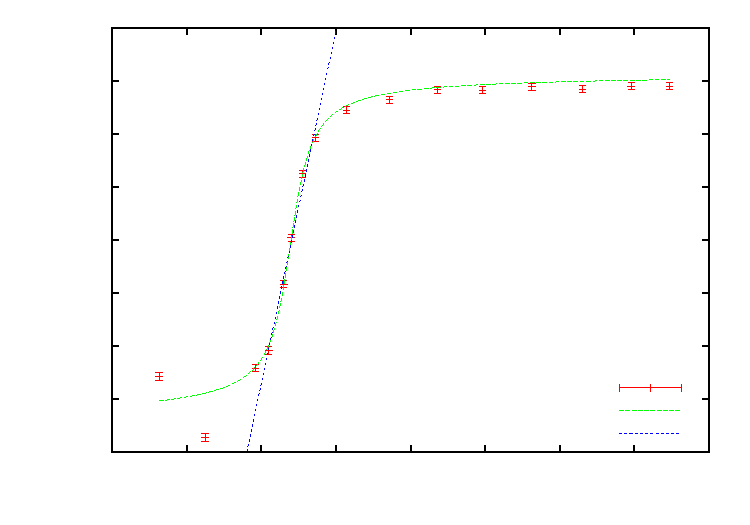
\includegraphics{phase}}%
    \gplfronttext
  \end{picture}%
\endgroup

	\caption{Phasenverschiebung des Serienresonanzkreises}
	\label{fig:phase}
\end{figure}

\begin{align}
\omega_\text{Phase}&=- \frac{b}{m}\\
\sigma_{\omega_\text{Phase}}&=\frac{1}{m^{2}} \cdot \sqrt{b^{2} \cdot \sigma_{m}^{2} + m^{2} \cdot \sigma_{b}^{2}}\\
\omega_\text{Phase}&=(1200 \pm 120)\,\si\hertz
\end{align}
\begin{figure}[!htb]
	\centering
	% GNUPLOT: LaTeX picture with Postscript
\begingroup
  \makeatletter
  \providecommand\color[2][]{%
    \GenericError{(gnuplot) \space\space\space\@spaces}{%
      Package color not loaded in conjunction with
      terminal option `colourtext'%
    }{See the gnuplot documentation for explanation.%
    }{Either use 'blacktext' in gnuplot or load the package
      color.sty in LaTeX.}%
    \renewcommand\color[2][]{}%
  }%
  \providecommand\includegraphics[2][]{%
    \GenericError{(gnuplot) \space\space\space\@spaces}{%
      Package graphicx or graphics not loaded%
    }{See the gnuplot documentation for explanation.%
    }{The gnuplot epslatex terminal needs graphicx.sty or graphics.sty.}%
    \renewcommand\includegraphics[2][]{}%
  }%
  \providecommand\rotatebox[2]{#2}%
  \@ifundefined{ifGPcolor}{%
    \newif\ifGPcolor
    \GPcolortrue
  }{}%
  \@ifundefined{ifGPblacktext}{%
    \newif\ifGPblacktext
    \GPblacktexttrue
  }{}%
  % define a \g@addto@macro without @ in the name:
  \let\gplgaddtomacro\g@addto@macro
  % define empty templates for all commands taking text:
  \gdef\gplbacktext{}%
  \gdef\gplfronttext{}%
  \makeatother
  \ifGPblacktext
    % no textcolor at all
    \def\colorrgb#1{}%
    \def\colorgray#1{}%
  \else
    % gray or color?
    \ifGPcolor
      \def\colorrgb#1{\color[rgb]{#1}}%
      \def\colorgray#1{\color[gray]{#1}}%
      \expandafter\def\csname LTw\endcsname{\color{white}}%
      \expandafter\def\csname LTb\endcsname{\color{black}}%
      \expandafter\def\csname LTa\endcsname{\color{black}}%
      \expandafter\def\csname LT0\endcsname{\color[rgb]{1,0,0}}%
      \expandafter\def\csname LT1\endcsname{\color[rgb]{0,1,0}}%
      \expandafter\def\csname LT2\endcsname{\color[rgb]{0,0,1}}%
      \expandafter\def\csname LT3\endcsname{\color[rgb]{1,0,1}}%
      \expandafter\def\csname LT4\endcsname{\color[rgb]{0,1,1}}%
      \expandafter\def\csname LT5\endcsname{\color[rgb]{1,1,0}}%
      \expandafter\def\csname LT6\endcsname{\color[rgb]{0,0,0}}%
      \expandafter\def\csname LT7\endcsname{\color[rgb]{1,0.3,0}}%
      \expandafter\def\csname LT8\endcsname{\color[rgb]{0.5,0.5,0.5}}%
    \else
      % gray
      \def\colorrgb#1{\color{black}}%
      \def\colorgray#1{\color[gray]{#1}}%
      \expandafter\def\csname LTw\endcsname{\color{white}}%
      \expandafter\def\csname LTb\endcsname{\color{black}}%
      \expandafter\def\csname LTa\endcsname{\color{black}}%
      \expandafter\def\csname LT0\endcsname{\color{black}}%
      \expandafter\def\csname LT1\endcsname{\color{black}}%
      \expandafter\def\csname LT2\endcsname{\color{black}}%
      \expandafter\def\csname LT3\endcsname{\color{black}}%
      \expandafter\def\csname LT4\endcsname{\color{black}}%
      \expandafter\def\csname LT5\endcsname{\color{black}}%
      \expandafter\def\csname LT6\endcsname{\color{black}}%
      \expandafter\def\csname LT7\endcsname{\color{black}}%
      \expandafter\def\csname LT8\endcsname{\color{black}}%
    \fi
  \fi
  \setlength{\unitlength}{0.0500bp}%
  \begin{picture}(7200.00,5040.00)%
    \gplgaddtomacro\gplbacktext{%
      \csname LTb\endcsname%
      \put(814,704){\makebox(0,0)[r]{\strut{} 0}}%
      \put(814,1383){\makebox(0,0)[r]{\strut{} 10}}%
      \put(814,2061){\makebox(0,0)[r]{\strut{} 20}}%
      \put(814,2740){\makebox(0,0)[r]{\strut{} 30}}%
      \put(814,3418){\makebox(0,0)[r]{\strut{} 40}}%
      \put(814,4097){\makebox(0,0)[r]{\strut{} 50}}%
      \put(814,4775){\makebox(0,0)[r]{\strut{} 60}}%
      \put(946,484){\makebox(0,0){\strut{} 0}}%
      \put(1678,484){\makebox(0,0){\strut{} 0.5}}%
      \put(2410,484){\makebox(0,0){\strut{} 1}}%
      \put(3142,484){\makebox(0,0){\strut{} 1.5}}%
      \put(3875,484){\makebox(0,0){\strut{} 2}}%
      \put(4607,484){\makebox(0,0){\strut{} 2.5}}%
      \put(5339,484){\makebox(0,0){\strut{} 3}}%
      \put(6071,484){\makebox(0,0){\strut{} 3.5}}%
      \put(6803,484){\makebox(0,0){\strut{} 4}}%
      \put(176,2739){\rotatebox{-270}{\makebox(0,0){\strut{}Spannung [V]}}}%
      \put(3874,154){\makebox(0,0){\strut{}$\omega$ [kHz]}}%
    }%
    \gplgaddtomacro\gplfronttext{%
      \csname LTb\endcsname%
      \put(5816,4602){\makebox(0,0)[r]{\strut{}$U$}}%
      \csname LTb\endcsname%
      \put(5816,4382){\makebox(0,0)[r]{\strut{}$U_{L+R}$}}%
      \csname LTb\endcsname%
      \put(5816,4162){\makebox(0,0)[r]{\strut{}$U_{C}$}}%
      \csname LTb\endcsname%
      \put(5816,3942){\makebox(0,0)[r]{\strut{}$U_C$-Fit}}%
    }%
    \gplbacktext
    \put(0,0){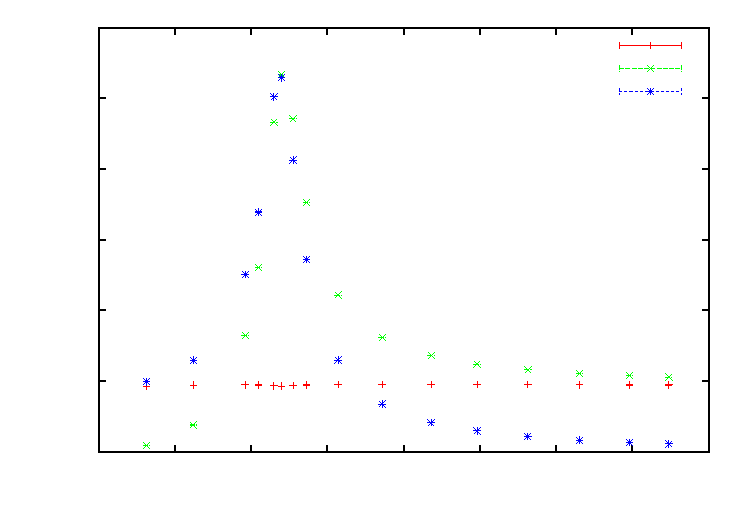
\includegraphics{spannungen}}%
    \gplfronttext
  \end{picture}%
\endgroup

	\caption{Teilspannungen des Serienresonanzkreises}
	\label{fig:teilU}
\end{figure}

\subsection{Parallelkreis}
\begin{figure}[!htb]
	\centering
	% GNUPLOT: LaTeX picture with Postscript
\begingroup
  \makeatletter
  \providecommand\color[2][]{%
    \GenericError{(gnuplot) \space\space\space\@spaces}{%
      Package color not loaded in conjunction with
      terminal option `colourtext'%
    }{See the gnuplot documentation for explanation.%
    }{Either use 'blacktext' in gnuplot or load the package
      color.sty in LaTeX.}%
    \renewcommand\color[2][]{}%
  }%
  \providecommand\includegraphics[2][]{%
    \GenericError{(gnuplot) \space\space\space\@spaces}{%
      Package graphicx or graphics not loaded%
    }{See the gnuplot documentation for explanation.%
    }{The gnuplot epslatex terminal needs graphicx.sty or graphics.sty.}%
    \renewcommand\includegraphics[2][]{}%
  }%
  \providecommand\rotatebox[2]{#2}%
  \@ifundefined{ifGPcolor}{%
    \newif\ifGPcolor
    \GPcolortrue
  }{}%
  \@ifundefined{ifGPblacktext}{%
    \newif\ifGPblacktext
    \GPblacktexttrue
  }{}%
  % define a \g@addto@macro without @ in the name:
  \let\gplgaddtomacro\g@addto@macro
  % define empty templates for all commands taking text:
  \gdef\gplbacktext{}%
  \gdef\gplfronttext{}%
  \makeatother
  \ifGPblacktext
    % no textcolor at all
    \def\colorrgb#1{}%
    \def\colorgray#1{}%
  \else
    % gray or color?
    \ifGPcolor
      \def\colorrgb#1{\color[rgb]{#1}}%
      \def\colorgray#1{\color[gray]{#1}}%
      \expandafter\def\csname LTw\endcsname{\color{white}}%
      \expandafter\def\csname LTb\endcsname{\color{black}}%
      \expandafter\def\csname LTa\endcsname{\color{black}}%
      \expandafter\def\csname LT0\endcsname{\color[rgb]{1,0,0}}%
      \expandafter\def\csname LT1\endcsname{\color[rgb]{0,1,0}}%
      \expandafter\def\csname LT2\endcsname{\color[rgb]{0,0,1}}%
      \expandafter\def\csname LT3\endcsname{\color[rgb]{1,0,1}}%
      \expandafter\def\csname LT4\endcsname{\color[rgb]{0,1,1}}%
      \expandafter\def\csname LT5\endcsname{\color[rgb]{1,1,0}}%
      \expandafter\def\csname LT6\endcsname{\color[rgb]{0,0,0}}%
      \expandafter\def\csname LT7\endcsname{\color[rgb]{1,0.3,0}}%
      \expandafter\def\csname LT8\endcsname{\color[rgb]{0.5,0.5,0.5}}%
    \else
      % gray
      \def\colorrgb#1{\color{black}}%
      \def\colorgray#1{\color[gray]{#1}}%
      \expandafter\def\csname LTw\endcsname{\color{white}}%
      \expandafter\def\csname LTb\endcsname{\color{black}}%
      \expandafter\def\csname LTa\endcsname{\color{black}}%
      \expandafter\def\csname LT0\endcsname{\color{black}}%
      \expandafter\def\csname LT1\endcsname{\color{black}}%
      \expandafter\def\csname LT2\endcsname{\color{black}}%
      \expandafter\def\csname LT3\endcsname{\color{black}}%
      \expandafter\def\csname LT4\endcsname{\color{black}}%
      \expandafter\def\csname LT5\endcsname{\color{black}}%
      \expandafter\def\csname LT6\endcsname{\color{black}}%
      \expandafter\def\csname LT7\endcsname{\color{black}}%
      \expandafter\def\csname LT8\endcsname{\color{black}}%
    \fi
  \fi
  \setlength{\unitlength}{0.0500bp}%
  \begin{picture}(7200.00,5040.00)%
    \gplgaddtomacro\gplbacktext{%
      \csname LTb\endcsname%
      \put(1254,704){\makebox(0,0)[r]{\strut{}-0.5}}%
      \put(1254,1156){\makebox(0,0)[r]{\strut{} 0}}%
      \put(1254,1609){\makebox(0,0)[r]{\strut{} 0.5}}%
      \put(1254,2061){\makebox(0,0)[r]{\strut{} 1}}%
      \put(1254,2514){\makebox(0,0)[r]{\strut{} 1.5}}%
      \put(1254,2966){\makebox(0,0)[r]{\strut{} 2}}%
      \put(1254,3419){\makebox(0,0)[r]{\strut{} 2.5}}%
      \put(1254,3871){\makebox(0,0)[r]{\strut{} 3}}%
      \put(1254,4324){\makebox(0,0)[r]{\strut{} 3.5}}%
      \put(1254,4776){\makebox(0,0)[r]{\strut{} 4}}%
      \put(1386,484){\makebox(0,0){\strut{} 0}}%
      \put(2083,484){\makebox(0,0){\strut{} 500}}%
      \put(2779,484){\makebox(0,0){\strut{} 1000}}%
      \put(3476,484){\makebox(0,0){\strut{} 1500}}%
      \put(4172,484){\makebox(0,0){\strut{} 2000}}%
      \put(4869,484){\makebox(0,0){\strut{} 2500}}%
      \put(5565,484){\makebox(0,0){\strut{} 3000}}%
      \put(6262,484){\makebox(0,0){\strut{} 3500}}%
      \put(6958,484){\makebox(0,0){\strut{} 4000}}%
      \put(484,2740){\rotatebox{90}{\makebox(0,0){\strut{}Impedanz [$\Omega$]}}}%
      \put(4172,154){\makebox(0,0){\strut{}Kreisfrequenz [Hz]}}%
    }%
    \gplgaddtomacro\gplfronttext{%
      \csname LTb\endcsname%
      \put(5971,4603){\makebox(0,0)[r]{\strut{}Messwerte}}%
    }%
    \gplbacktext
    \put(0,0){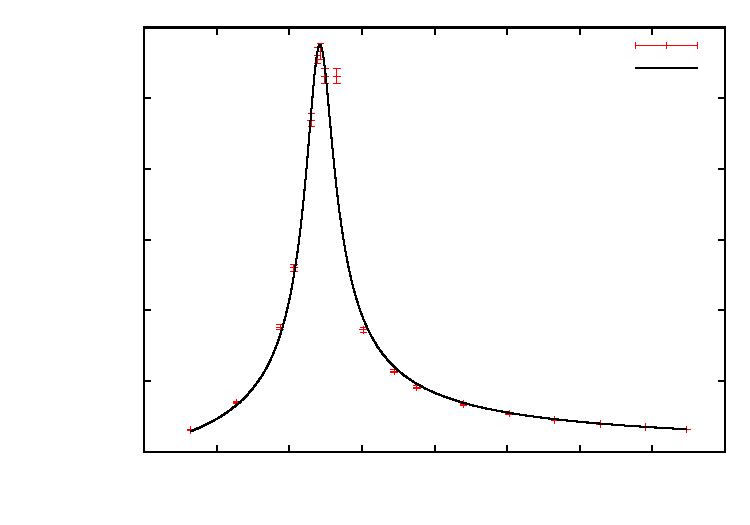
\includegraphics{messung3}}%
    \gplfronttext
  \end{picture}%
\endgroup

	\caption{Impedanz des Parallelkreises als Funktion der Kreisfrequenz}
	\label{fig:messung3}
\end{figure}

Aus Fit von Messung 3:
\begin{align}
	R &= (68\pm 5)\si{\kilo\ohm}\\
	L &= (370 \pm 10)\si{\milli\henry}\\
	C &= (1.88  \pm 0.05) \si{\micro\farad}
\end{align}

Daraus ergibt sich eine Resonanzfrequenz
\begin{align}
	\omega_R=(1200 \pm 20)\,\si{\hertz} \,.
\end{align}


\section{Diskussion}
\label{sec:diskussion}

\bibliography{literatur}
\bibliographystyle{babalpha}
\end{document}
